\subsection{Dynkin 图}

依照通常的语言滥用，我们称具有以下性质的一对 \((\Gamma, f)\) 为赋范图：

\begin{enumerate}
\def\labelenumi{\arabic{enumi})}
\item
  \(\Gamma\) 是一个图（称为 \((\Gamma, f)\) 的底图）。
\item
  若 E 表示有序对 \((i,j)\) 所成的集合，其中 \(\{i,j\}\) 是 \(\Gamma\) 的一条边，则 f 是从 E 到 R 的映射，并且有 \(f(i,j)f(j,i)=1\)（对所有 \((i,j)\in\mathbf{E}\)）。
\end{enumerate}

赋范图的同构概念是显然的。

设 R 是实向量空间 V 中的一个约化根系。我们将与之关联一个赋范图 \((X, f)\)，称为 R 的 Dynkin 图。X 的顶点将是 W(R) 在 \(\{B\} \times B\) 的并集（其中 B 为 R 的基集）中的轨道集 I 的元素。若 \(N = (n_{ij})_{i,j \in I}\)（分别为 \(M = (m_{ij})_{i,j \in I}\)）是 R 的典范 Cartan 矩阵（分别为 Coxeter 矩阵）（\(\S\) 1，第 5 号，备注 7），则 X 的两个顶点 i 和 j 相连，当且仅当 \(n_{ij} \neq 0\)，并置

\[
f (i, j) = \frac {n _ {i j}}{n _ {j i}}.
\]

由于 \(n_{ij} = 0\) 蕴含 \(n_{ji} = 0\)，这定义了一个赋范图 (X. f)。

设 \((x|y)\) 是 V 上在 W(R) 下不变的标量积，令 \(B = (\alpha_i)_{i \in I}\) 为 R 的一组按典范方式编号的基。第 1 节第 1 号的公式 (7) 和 (9) 表明，图 X 的顶点 i 和 j 相连，当且仅当

\[
(\alpha_ {i} | \alpha_ {j}) \neq 0
\]

并且

\[
f (i, j) = \frac {\left(\alpha_ {j} \mid \alpha_ {i}\right)}{\left(\alpha_ {j} \mid \alpha_ {j}\right)}.
\]

根据第 1 节第 3 号和第 5 号的结果，除交换 \(i\) 和 \(j\) 外，只有以下可能性：

\begin{enumerate}
\def\labelenumi{\arabic{enumi})}
\item
  \(i\) 和 \(j\) 不相连；\(n_{ij} = n_{ji} = 0\)；\(m_{ij} = 2\)；
\item
  \(f(i,j) = f(j,i) = 1; n_{ij} = n_{ji} = -1; m_{ij} = 3;\)
\item
  \(f(i,j) = 2\)，\(f(j,i) = 1/2\)；\(n_{ij} = -2\)。\(n_{ji} = -1\)；\(m_{ij} = 4\)；
\end{enumerate}

\[
f (i, j) = 3, f (j, i) = 1 / 3: n _ {i j} = - 3, n _ {j i} = - 1; m _ {i j} = 6.
\]

由此可见，Dynkin 图 R 确定 R 的 Cartan 矩阵和 Coxeter 矩阵，因而将 R 确定到同构为止。更精确地说，第 1 节第 5 号命题 15 的推论蕴含以下结果：

命题 1. 设 \(R_{1}\) 和 \(R_{2}\) 是向量空间 \(V_{1}\) 和 \(V_{2}\) 中的两个约化根系。设 \(B_{1} = (\alpha_{i})_{i \in I_{1}}\) 和 \(B_{2} = (\alpha_{i})_{i \in I_{2}}\) 分别为 \(R_{1}\) 和 \(R_{2}\) 的按典范方式编号的基。设 \(\lambda\) 是从 \(R_{1}\) 的 Dynkin 图到 \(R_{2}\) 的 Dynkin 图的同构。则存在唯一的从 \(V_{1}\) 到 \(V_{2}\) 的同构，将 \(R_{1}\) 变为 \(R_{2}\)，并且将 \(\alpha_{i}\) 变为 \(\alpha_{\lambda(i)}\)（对所有 \(i \in I_{1}\)）。

显然，R 的一个自同构定义 R 的 Dynkin 图的一个自同构，从而定义从群 A(R) 到 R 的 Dynkin 图自同构群的同态 \(\varphi\)。

推论。同态 \(\varphi\) 通过取商定义了从群 A(R)/W(R) 到 R 的 Dynkin 图自同构群的一个同构。

显然，\(\varphi(g) = \operatorname{Id}\)（对所有 \(g \in W(R)\)）。另一方面，命题 1 表明，存在一个同构 \(\psi\)，它从 \(R\) 的 Dynkin 图同构群映到 \(E\)，而 \(A(R)\) 中固定给定基 \(B\)（属于 \(R\)）的元素组成此子群，并且满足 \(\varphi \circ \psi = \operatorname{Id}\)。由于 \(A(R)\) 是 \(E\) 与 \(W(R)\) 的半直积（第 1 节，第 5 号，命题 16），推论得证。

实际上，Dynkin 图 \((X, f)\) 用由节点和边组成的图表示如下。节点对应于 X 的顶点；在上述情形 1）、2）、3）和 4）中，分别用 0、1、2 或 3 条边连接对应于两个不同顶点 i 和 j 的两个节点（除交换 i 和 j 外）。此外，在情形 3）和 4）中，即当 \(f(i, j) > 1\)，或根 \(\alpha_{1}\) 与 \(\alpha_{j}\) 不正交且长度不同时，在连接对应于 i 和 j 的节点的双边或三边上放置不等号 \textgreater{}，方向指向对应于 j 的节点（即较短的根）：

\[
\underset {i} {\longrightarrow} \underset {j} {\longrightarrow} \quad (\text { for   } f (i, j) = 2), \quad \underset {i} {\longrightarrow} \underset {j} {\longrightarrow} \quad (\text { for   } f (i, j) = 3).
\]

显然，可以从此图恢复 Dynkin 图 \((X, f)\)。

注意，与 W(R) 的 Coxeter 图对应的图可以从与 R 的 Dynkin 图对应的图得到：保留节点和单边，并将双边（分别为三边）替换为上方标有数字 4（分别为 6）的边。反过来，给定 W(R) 的 Coxeter 图，可以使用此过程的逆过程恢复与 R 的 Dynkin 图对应的图，但双边或三边上的不等号除外。因此定理 1 立即给出可能的 Dynkin 图列表。更精确地说：

定理 3. 若 R 是不可约约化根系，则其 Dynkin 图同构于以下图示中的某一个图：

\pandocbounded{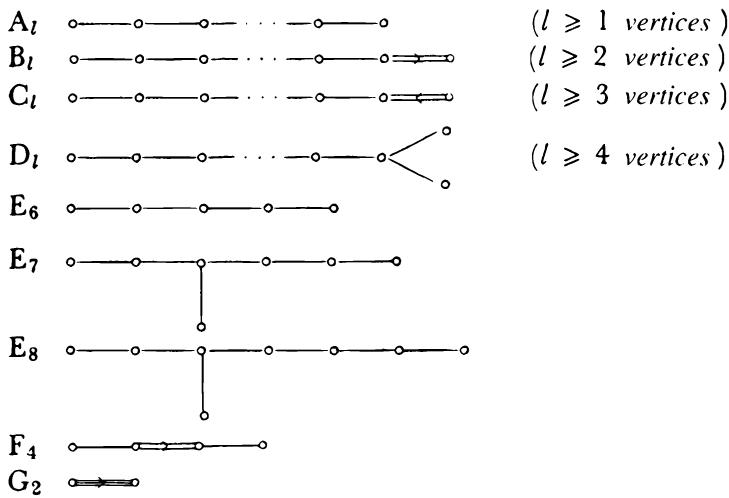
\includegraphics[keepaspectratio]{images/part002_c37a5a77.jpg}}

这些图中任意两个都不同构，并且存在不可约约化根系，使每一个图（在同构意义下）都成为其 Dynkin 图。

第一个断言立即由定理 1、上述备注、图 \(H_{3}\)、\(H_{4}\) 和 \(I_{2}(p)\) 的 Coxeter 群（当 p = 5 及 \(p \geqslant 7\) 时）不是晶体群这一事实，以及与 Coxeter 图 \(F_{4}\)（分别为 \(G_{2}\)）对应的 Dynkin 图的双边（分别为三边）的两种可能不等号给出同构 Dynkin 图这一事实得到。第二个断言是显然的，第三个断言将由对每一种类型明确构造一个不可约约化根系而得出；这一构造将在第 5 至 13 号中进行。

备注。1）图 \(A_{1}\) 退化为一个节点；也记为 \(B_{1}\) 或 \(C_{1}\)。图 \(B_{2}\) 也记为 \(C_{2}\)。图 \(A_{3}\) 也记为 \(D_{3}\)。最后，\(D_{2}\) 表示由两个不相连节点组成的图。（这些约定源于相应根系的性质，参见第 5 至 8 号。）

\begin{enumerate}
\def\labelenumi{\arabic{enumi})}
\setcounter{enumi}{1}
\tightlist
\item
  若 \((X, f)\) 是约化根系 R 的 Dynkin 图，则对偶根系的 Dynkin 图可与 \((X, f^{-1})\) 认同。换言之，与 \(R^{\prime}\) 的 Dynkin 图对应的图可以从与 R 的 Dynkin 图对应的图得到，只需反转不等号。若 R 不可约，则可见 R 与 \(R^{\prime}\) 同构，除非 R 是 \(B_{l}\) 型或 \(C_{l}\) 型；在这两种情形下，\(R^{\prime}\) 分别是 \(C_{l}\) 型或 \(B_{l}\) 型。
\end{enumerate}

